\section{Neuronale Netze}
Ein neuronales Netz ist ein Zusammenschluss aus mehreren Perceptronen in verschiedenen Layern. Als Beispiel sei an
dieser Stelle die Abbildung \ref{fig:07_neuronal_network} gegeben. Dieses wird ebenso verwendet, um die Ableitungskette
für ein Gewicht in diesem Fall zu zeigen. Anzumerken sei hier, dass die Kombination der gewichteten Summem mit der
Aktivierungsfunktion ein Neuron darstellt.

\begin{figure}[h!]
    \begin{center}
        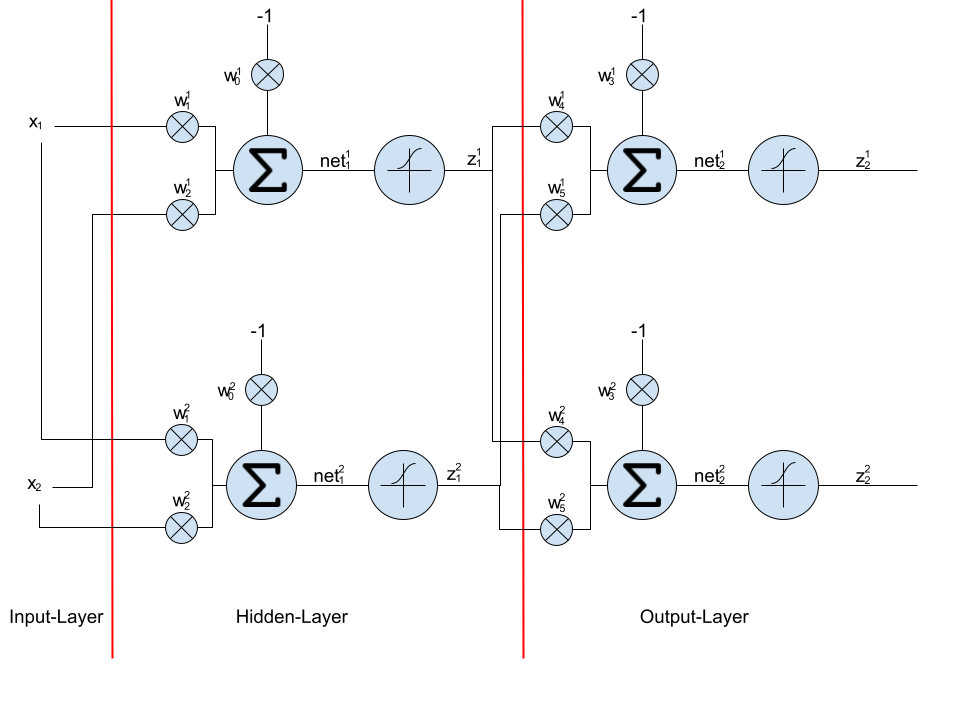
\includegraphics[width=1\linewidth]{../common/01_neuronal_network/00_resources/02_neuronales_netz.png}
    \end{center}
    \caption{Ein neuronales Netz mit einem Hidden-Layer}
    \label{fig:07_neuronal_network}
\end{figure}

\subsection{Lernverfahren mit Gradientenabstieg}
Wie beim Perceptron auch soll nun an dieser Stelle die Komponente des Gradienten für das Gewicht $w_1^1$ gezeigt
werden. Für dieses Beispiel wird die Abbildung \ref{fig:07_neuronal_network} hinzugezogen.
Die Fehlerfunktion ist wie beim Perceptron dieselbe $P_{err} = - \frac{1}{2} \cdot \sum_i^2 (d^i - z_2^i)^2$.
In diesem Fall steht die Komponente $i$ für den Index und die $2$ für den Layer.
Folgende Werte sind bekannt:
\begin{align}
    P_{err} = - \frac{1}{2} \cdot \sum_i^2 (d^i - z_2^i)^2\\
    net_1^1 = x_1 \cdot w_1^1 + x_2 \cdot w_2^1 - w_0^1\\
    z_1^1 = \frac{1}{1 + e^{-net_1^1}}\\
    net_1^2 = x_1 \cdot w_1^2 + x_2 \cdot w_2^2 - w_0^2\\
    z_1^2 = \frac{1}{1 + e^{-net_1^2}}\\
    net_2^1 = z_1^1 \cdot w_4^1 + z_1^2 \cdot w_5^1 - w_3^1\\
    z_2^1 = \frac{1}{1 + e^{-net_2^1}}\\
    net_2^2 = z_1^1 \cdot w_4^2 + z_1^2 \cdot w_5^2 - w_3^2\\
    z_2^2 = \frac{1}{1 + e^{-net_2^2}}
\end{align}
Der Gradient für die Gewichte setzt sich wie nachfolgend zusammen:
\begin{align}
    \vec{\nabla} = (w_0^1, w_1^1, w_2^1, w_0^2, w_1^2, w_2^2, w_3^1, w_4^1, w_5^1, w_3^2, w_4^2, w_5^2)
\end{align}
Die Korrektur in einem Schritt kann wiederum über den Vektor der Gewichte $\vec{w}$ erfolgen.
\begin{align}
    \vec{w}_{neu} = \vec{w}_{alt} + \lambda \cdot \vec{\nabla}
\end{align}
Wie bereits erwähnt wird nun nur die Komponente $w_1^1$ aus dem Vektor $\vec{\nabla}$
berücksichtigt. Um diesen herzuleiten, müssen alle Pfade zum Gewicht berücksichtigt werden.
In dem Fall gibt es zwei Pfade:
\begin{multline}
    P_{err} = - \frac{1}{2} \cdot (d^1 - z_2^1(net_2^1(w_4^1 \cdot z_1^1(net_1^1(w_1^1 \cdot x_1, w_2^1 \cdot x_2, -w_0^1)), z_1^2 \cdot w_5^1, -w_3^1)))^2 + (d^2 - z_2^2)\\
    P_{err} = - \frac{1}{2} \cdot (d^2 - z_2^2(net_2^2(w_4^2 \cdot z_1^1(net_1^1(w_1^1 \cdot x_1, w_2^1 \cdot x_2, -w_0^1)), z_1^2 \cdot w_5^2, -w_3^2)))^2 + (d^1 - z_2^1)
\end{multline}
Dementspreched werden die beiden Pfade für die Komponente des Gradienten für $w_1^1$ berücksichtigt.
\begin{multline}
    \frac{\delta P_{err}}{\delta w_1^1} = \frac{\delta P_{err}}{\delta z_2^1(w_1^1)} \cdot \frac{\delta z_2^1(w_1^1)}{\delta net_2^1(w_1^1)} \cdot \frac{\delta net_2^1(w_1^1)}{\delta z_1^1(w_1^1)} \cdot \frac{\delta z_1^1{w_1^1}}{\delta net_1^1(w_1^1)} \cdot \frac{\delta net_1^1(w_1^1)}{\delta w_1^1} +\\
    \frac{\delta P_{err}}{\delta z_2^2(w_1^1)} \cdot \frac{\delta z_2^2(w_1^1)}{\delta net_2^2(w_1^1)} \cdot \frac{\delta net_2^2(w_1^1)}{\delta z_1^1(w_1^1)} \cdot \frac{\delta z_1^1{w_1^1}}{\delta net_1^1(w_1^1)} \cdot \frac{\delta net_1^1(w_1^1)}{\delta w_1^1}
\end{multline}
Anders ausgedrückt lautet demnach die Komponente:
\begin{multline}
    w_{1,korr}^1 = (d^1 - z_2^1) \cdot z_2^1(1 - z_2^1) \cdot w_4^1 \cdot z_1^1(1 - z_1^1) \cdot x_1 +\\
    (d^2 - z_2^2) \cdot z_2^2(1 - z_2^2) \cdot w_4^2 \cdot z_1^1(1 - z_1^1) \cdot x_1
\end{multline}
An dieser Stelle sei nun angemerkt, dass dieses Verfahren durchaus funktioniert, jedoch wachsen die Ableitungsterme
exponentiell mit der Anzahl Neuronen in den Layern. Aus diesem Grund ist der Gradientenabstieg so nicht brauchbar in
der Praxis. Was jedoch auffällt ist die Tatsache, dass einmal berechnete Ableitungsketten wiederverwendet werden können.
Gedanklich kann an dieser Stelle z.B. die Ableitungskette für $w_2^1$ hinzugezogen werden. Man erkennt relativ schnell,
dass viele Berechnung, welche schon für $w_1^1$ gemacht wurden, wiederauftreten. Auf Grundlage dieser Idee der
dynamischen Programmierung wurde der Backpropagation Algorithmus entwickelt.

\subsection{Lernverfahren mit Backpropagation}
Der grosse Vorteil dieses Verfahrens ist die Berechnungszeit, welche im Vergleich zum reinen Gradientenabstieg nur noch
linear mit den Anzahl der Gewichte wächst. So werden einmal berechnete Ableitungsketten gespeichert und wiederverwendet.

\subsection{XOR und die Lösung}